 \documentclass[11pt]{article}

\usepackage{latexsym}
\usepackage{amssymb}
\usepackage{amsthm}
\usepackage{amscd}
\usepackage{amsmath}
\usepackage{tikz}
\usepackage{graphicx}
\usepackage{enumerate}
\usepackage{pdfpages}


\newcommand{\ZZ}{\mathbb{Z}}

\setlength{\evensidemargin}{1in}
\addtolength{\evensidemargin}{-1in}
\setlength{\oddsidemargin}{1.5in}
\addtolength{\oddsidemargin}{-1.5in}
\setlength{\topmargin}{1in}
\addtolength{\topmargin}{-1.5in}

\setlength{\textwidth}{16cm}
\setlength{\textheight}{23cm}

\newcommand{\rook}{\hspace{-.1cm}\amalg\hspace{-.15cm}\bar{}}
\newcommand{\Stab}{\mathrm{Stab}}
\newcommand{\FF}{\mathbb{F}}


\begin{document}
\begin{center}
\section*{William Daniels}
\section*{CSCI 4630}
\subsection*{HW \#1}
\subsection*{February 1st}
\end{center}
\vspace{.25cm}
\begin{enumerate}
\item \textbf{The Missionaries and Cannibals problem}\\\\
Three Missionaries and three cannibals find themselves on one side of a river. They have agreed that they would all like to get to the other side. But the missionaries are not sure waht else the cannibals have agreed to. So the missionaries want to manage the trip across the river in such a way that the number of missionaries on either side of the river is never less than the number of cannibals who are on the same. The only boat available holds on two people at a time. hw can everyone get across the river without the missionaries rising begin eaten. \\\\
\textbf{Solution:}\\\\
First, we establish our state space: 
state space $(c, m)$:
\begin{align*}
&c\text{ is the number of cannibals on side B of the river}\\
&m \text{ is the number of cannibals on side B of the river}\\
\end{align*}
Now, the heuristic function for this problem is determined as follows: For each missionary on the 'B' side of the river, add 1, for each missionary on the 'A' side of the river, subtract one. For each cannibal on side 'B' of the river, add 1, and for each cannibal on side 'A' of the river, subtract 1. If there are more cannibals than missionaries on either side of the river, subtract 1 for each cannibal above the number of missionaries on each side of the river. If there are no missionaries on a side, don't add anything. If the number of missionaries and cannibals on both sides of the river is the same, add 1. 
With that heuristic in mind, lets proceed to the solution. The idea, is that the state space simply allows for us to represent the number of cannibals and missionaries on side B of the river, and based upon this, the movement patterns can be discerned. 
The derivation result of the number of missionaries and cannibals on side B of the river looks like the following: 
\begin{align*}
&\rightarrow (1,1)\\
&\rightarrow (3,0)\\
&\rightarrow (2,2)\\
&\rightarrow (1,3)\\
&\rightarrow (2,3)\\
&\rightarrow (3,3)\\
\end{align*}
Now, this corresponds to the following pattern of concluded movement, using the following production rule: 
\textbf{Production rules}:\\\\
\begin{enumerate}[(a)]
\item move (u, v):
$$(c, m) \rightarrow ( c + u, m +v)$$
\end{enumerate}
Now, with that in mind, the following moves apply
\begin{enumerate}[(1)]
\item move $(1,1)$
\item move $(0,-1)$
\item move $(2,0)$
\item move $(-1, 0)$
\item move $(0,2)$
\item move $(-1,-1)$
\item move $(0,2)$
\item move $(-1,0)$
\item move $(2,0)$
\item move $(-1,0)$
\item move $(2,0)$
\end{enumerate}

Below is the state diagram with the heuristic applied to every state: 
\begin{figure}[ht!]
\centering
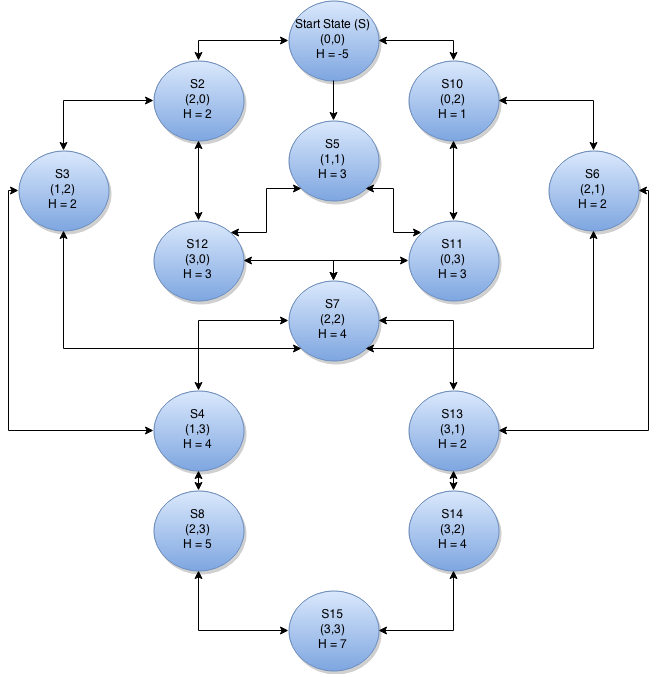
\includegraphics[width=100mm]{HW1StateDiagram.png}
\caption{State Diagram for Missionaries and Cannibals problem \label{overflow}}
\end{figure}

\item \textbf{The Tower of Hanoi}\\\\
Somewhere near Hanoi there is a monastery whose monks devote their lives to
a very important task. In their courtyard are three tall posts. On these posts is a
set of sixty-four disks, each with a hole in the center and each of a different
radius. When the monastery was established, all of the disks were on one of the
posts, each disk resting on one just larger than it. The monks' task is to move
all the disks to one of the other pegs. Only one disk may be moved at a time,
and all the other disks must be on one of the pegs. In addition, at no time
during the process may a disk be placed on top of a smaller disk. The third peg
can, of course, be used as a temporary resting place for disks. What is the
quickest way for monks to accomplish their mission?
 Even the best solution to this problem will take the monks a very long time.
This is fortunate, since legend has it that the world will end when they have finished.\\\\
\textbf{Solution:}\\\\
In order to properly assess this problem, we will use a much smaller set size (number of discs $(n) = 3$) In order to create a manageable problem. 
First, we establish our state space: \\
state space $(w, x, y, z)$:
\begin{align*}
&w - \text{The number of the smallest disc of the first tower}\\
&x - \text{The number of the smallest disc of the second tower} \\
&y - \text{The number of the smallest disc of the third tower} \\
\end{align*}
Production Rules: 
\begin{enumerate}
\item  moveFromFirstToThird $(u):$\\
$$(w, x, y) \rightarrow (w - u, x, y+u)$$
\item  moveFromFirstToSecond $(u):$\\
$$(w, x, y) \rightarrow (w - u, x+u, y)$$
\item  moveFromThirdToFirst $(u):$\\
$$(w, x, y) \rightarrow (w + u, x, y- u)$$
\item  moveFromThirdToSecond $(u):$\\
$$(w, x, y) \rightarrow (w, x+u, y-u)$$
\item  moveFromSecondtToThird $(u):$\\
$$(w, x, y) \rightarrow (w, x - u, y+u)$$
\item  moveFromSecondToFirst $(u):$\\
$$(w, x, y) \rightarrow (w + u, x, y - u)$$
\end{enumerate}

Now, the heuristic we'll apply will be relatively simple. count the number of discs on tower 1, subtract 1 for each disc.Finally, count the number of discs on tower 3, add 1 for each. For each disc on tower 3 that is in it's final, correct position, add 2.
The state diagram with this heuristic applied, looked like the following: 
\begin{figure}[ht!]
\centering
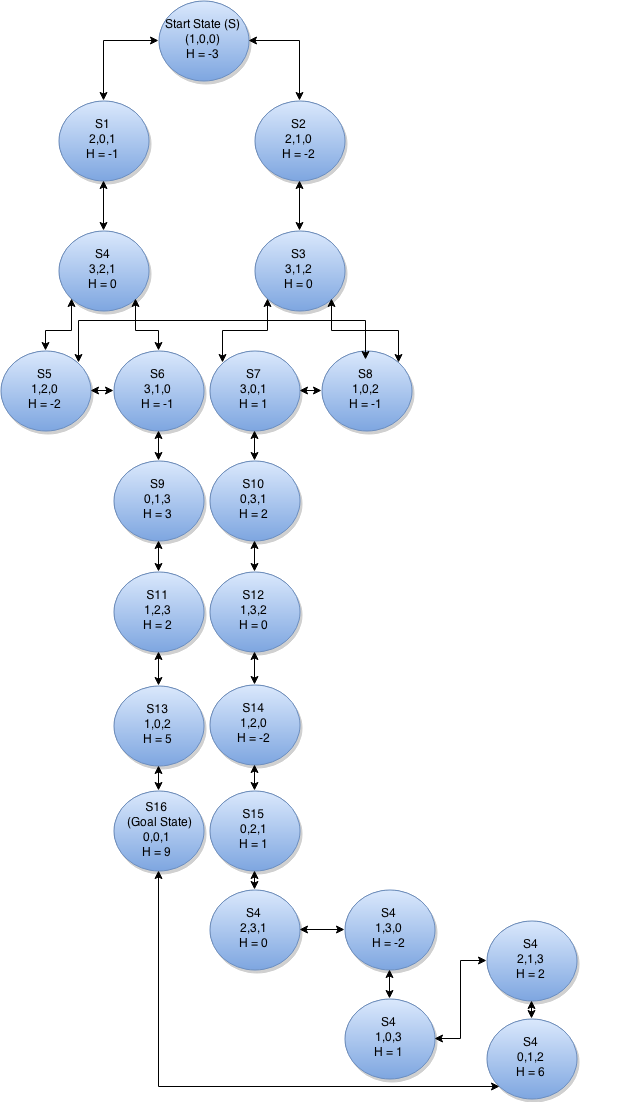
\includegraphics[width=100mm]{HanoiTower.png}
\caption{State Diagram for Towers of Hanoi \label{overflow}}
\end{figure}

Which then provides an optimal (shortest) path solution of: 
\begin{enumerate}[(1)]
\item moveFromFirstToThird $(1)$
\item moveFromFirstToSecond $(2)$
\item moveFromThirdToSecond $(1)$
\item moveFromFirstToThird $(3)$
\item moveFromSecondToFirst $(1)$
\item moveFromSecondToThird $(2)$
\item moveFromFirstToThird $(1)$
\end{enumerate}

So, simply 7 steps in order to solve the problem for 3 discs. This pattern, of always moving the top disc of tower 1  to the third tower, taking the next disc of tower 1, moving it to the temporary tower, then taking the third disc and moving it to the third tower, then re-stacking the other discs on top of the third tower, can be repeated for any size n. The only difference comes when you have enough you have to use the same pattern, but to stack the discs on tower 2, allowing the bottom of tower 3 to open up. 



\end{enumerate}



\end{document}

